\section{El paquete de Python y los bloques que lo conforman}
Python es un lenguaje de código abierto, con una comunidad activa de colaboradores y usuarios que comparten su software para que otros desarrolladores lo utilicen. Son colaboradores aquellos que comparten sus códigos o scripts, en forma de paquetes en el Python Packaging Index (PyPI). Los paquetes son similares a directorios de un sistema de archivos ya que estos permiten separar el código de forma jerárquica \cite{Paquetes}. De acuerdo con la documentación oficial, existen 3 tipos de paquetes:
\begin{itemize}
    \item \textbf{Paquetes regulares:} Son implementados como un directorio o carpeta, que contiene un archivo \mintinline{Python}{init__.py}. Cuando se importa un paquete regular, este archivo \mintinline{Python}{init__.py} se ejecuta implícitamente y los objetos que define, están vinculados a nombres en el espacio de nombres del paquete. Por ejemplo, la siguiente disposición del sistema de archivos define un paquete "parent" de nivel superior con tres sub-paquetes:
\begin{figure}[H]
    \centering
    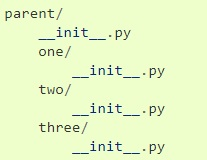
\includegraphics[scale = 0.8]{Recursos/paqueteRegular.jpg}
    \caption{Organización de directorios de un paquete regular}
    \label{PaqueteRegular}
\end{figure}
Cuando se requiere emplear un paquete es necesario primero importarlo; por lo que al importar parent.one (Ver Figura \ref{PaqueteRegular}) se ejecutará implícitamente \mintinline{Python}{parent/__init__.py} y \mintinline{Python}{parent/one/__init__.py}. 
\item \textbf{Paquetes de espacio de nombre (namespace package):} Pertenecen a esta categoría aquellos paquetes compuestos por un conjunto de archivos en un único directorio, donde cada grupo de archivos contribuye con un sub-paquete del paquete padre. A diferencia de los paquetes regulares, los conjuntos pueden estar en diferentes lugares del sistema de archivos, pueden estar en archivos .zip, en la red o cualquier otro lugar que Python busque durante la importación.
\\
Un ejemplo en donde se separa el paquete en dos distribuciones utilizando namespaces sería:
\begin{figure}[H]
    \centering
    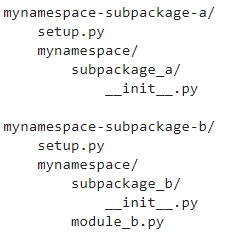
\includegraphics{Recursos/namespacePaquete.jpg}
    \caption{Organización de directorios de un paquete de espacios de nombre}
    \label{namespacePaquete}
\end{figure}
La forma de organizar el paquete utilizada en la Figura \ref{namespacePaquete} no es la única, existen otras formas donde el fichero setup.py, se encuentra en la raíz del paquete, como es el caso de los paquetes con namespace implícito \cite{PEP420}.  El fichero setup.py es aquel que permite la construcción, distribución e instalación de módulos.
\item \textbf{Paquete de importaciones relativas:} Basados en puntos iniciales. Un punto inicial indica una importación relativa, empezando por el paquete actual. Dos o más puntos iniciales indican una importación relativa a los elementos primarios del paquete actual, un nivel por punto después del primero. Por ejemplo, dado el siguiente diseño de paquete:
\begin{figure}[H]
    \centering
    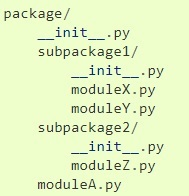
\includegraphics{Recursos/paqueteImportacionRelativa.jpg}
    \caption{Organización de directorios de un paquete de importaciones relativas}
    \label{paqueteIR}
\end{figure}
En \mintinline{Python}{subpackage1/moduleX.py} o \mintinline{Python}{subpackage1/__init__.py}, las siguientes son importaciones relativas válidas:
\begin{figure}[H]
    \centering
    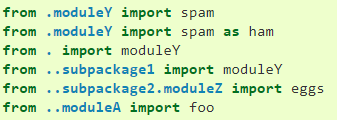
\includegraphics{Recursos/importarRelativamente.png}
    \caption{Ejemplo de importaciones relativas}
    \label{importarIR}
\end{figure}
\end{itemize}
\subsection{Módulos}
Se conoce como modulo a todo fichero o script de Python cuya extensión es .py. Separar el código en módulos permite facilitar el mantenimiento del programa a medida que crezca. Algunos aspectos a tomar en cuenta sobre los módulos serían:
\begin{itemize}
    \item Pueden contener tanto declaraciones ejecutables como definiciones de funciones. Estas declaraciones están pensadas para inicializar el módulo. Se ejecutan únicamente la primera vez que el módulo se encuentra en una declaración import\cite{ModuloPython}.
    \item Cada módulo tiene su propio espacio de nombres, el cual es usado como espacio de nombres global para todas las funciones definidas en su interior.
    \item Para optimizar la importación de módulos el autor del modulo deberá proveer un índice explícito del paquete. Esto se logra cuando el código en el archivo \mintinline{Python}{__init__.py} de un paquete define una lista llamada \mintinline{Python}{__all__.py}, dicha lista debe poseer los nombres de módulos que deberían ser importados cuando se hace \mintinline{Python}{from package import *}\cite{ModuloPython}.
\end{itemize}
\subsection{Tipos de  scripts de configuración del paquete}
\subsubsection{Distutils}
Es un paquete de Python que da soporte, para la creación, distribución e instalación de módulos, los módulos pueden ser hechos únicamente en Python o escritos en C. Distutils como paquete presenta las siguientes funcionalidades:
\begin{itemize}
    \item Soporte para declarar dependencias del proyecto, siendo las dependencias aquellos paquetes o módulos externos necesarios para el funcionamiento del proyecto.
    \item Mecanismos adicionales para configurar cuáles archivos incluir en lanzamientos de código fuente, esto se logra mediante el uso de sistemas de control de versiones.
    \item La capacidad de generar, automáticamente, ejecutables de línea de comandos de Windows en el momento de la instalación, en lugar de tener que compilarlos previamente.
    \item Comportamiento consistente en todas las versiones de Python soportadas por el paquete.
\end{itemize}
Un ejemplo de como estructurar el archivo setup.py que maneja Distutils sería:
\begin{figure}[H]
    \centering
    \begin{minted}{Python}
		from distutils.core import setup
		setup(name='Distutils',
                version='1.0',
                description='Python Distribution Utilities',
                author='Greg Ward',
                author_email='gward@python.net',
                url='https://www.python.org/sigs/distutils-sig/',
                packages=['distutils', 'distutils.command'],)
	\end{minted}
    \caption{Ejemplo de archivo setup.py utilizando el paquete Distutils}
    \label{ejDistutils}
\end{figure}
En la Figura \ref{ejDistutils} es importante resaltar la opción ``packages'' debido a que esta le dice a Distutils que procese (compile, distribuya, instale, etc.) todos los módulos de Python que se encuentran en cada paquete mencionado en la lista de "packages".
\subsubsection{Setuptools}
Es un paquete que contiene una serie de mejoras a las capacidades de Distutils, cuya cualidad principal es permitir que los desarrolladores puedan distribuir paquetes de forma más sencilla, con especial énfasis en paquetes que posean dependencias externas. Esto no implica que distutils sea obsoleto, puesto que setuptools aun se encuentra en desarrollo. A diferencia de su contra parte, las configuraciones requieren de al menos 2 archivos y un paquete, el archivo pyproject.toml; es aquel donde se debe declarar que se empleara Setuptools, este archivo debe poseer la siguiente estructura:
\begin{figure}[H]
    \centering
    \begin{minted}{Python}
		[build-system]
        requires = ["setuptools", "wheel"]
        build-backend = "setuptools.build_meta"
	\end{minted}
    \caption{Ejemplo de archivo pyproject.toml}
    \label{pyproject.toml}
\end{figure}
El archivo setup.cfg es el reemplazo al archivo setup.py y puede conformarse de la siguiente manera:
\begin{figure}[H]
    \centering
    \begin{minted}{Python}
		[metadata]
        name = "mypackage"
        version = 0.0.1

        [options]
        packages = "mypackage"
        install_requires =
        requests
        importlib; python_version == "2.6"
        
        [options.entry_points]
        console_scripts =
        main = mypkg:some_func
	\end{minted}
    \caption{Ejemplo de archivo setup.cfg}
    \label{setup.cfg}
\end{figure}
Como se puede ver en la Figura \ref{setup.cfg} el archivo es bastante similar en estructura al fichero setup.py; no obstante, tiene varias ventajas, ya que los elementos que pertenecen a la opción \mintinline{Python}{install_requires}, son directamente las dependencias del paquete, e incluso al momento de instalar un paquete externo, setuptools actualiza las dependencias necesarias. Para proyectos muy grandes es posible automatizar la busqueda de paquetes, con el fin de que no sea necesario declarar cada paquete en el fichero setup.cfg. 
Las herramientas de configuración admiten la creación automática de scripts tras la instalación mediante "\mintinline{Python}{options.entry_points}". Un paquete que emplee setuptools debe poseer la siguiente estructura de directorios:
\begin{figure}[H]
    \centering
    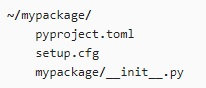
\includegraphics{Recursos/estructuraSetupTools.jpg}
    \caption{Estructura de paquete mediante setuptools}
    \label{estructuraSetupTools}
\end{figure}
El último elemento que requiere Setuptools es el paquete pep517, el cual se puede instalar mediante el instalador de paquetes de python "pip", posteriormente se debe invocar con el comando \mintinline{Python}{python -m pep517.build}.
\subsection{El paquete wheel}
Es un proyecto compatible con distutils y setuptools, que produce un formato de empaquetado binario multiplataforma (llamado ``wheels'' o ``wheel files'' y definido en PEP 427) es decir; la función de wheels es permitir la distribución de paquetes sin importar el sistema operativo empleado \cite{wheel}.
\subsection{Pruebas de regresión mediante modulo unittest}
El objetivo de las pruebas de regresión implementadas mediante el modulo unittest, es probar situaciones donde el codigo deje de funcionar, para encontrar errores en el mismo y solventar problemas en el software, de acuerdo con la documentación oficial existen una serie de pautas a seguir para ejecutar dichas pruebas, las más importantes en el caso del software a desarrollar son:
\begin{itemize}
    \item El conjunto de pruebas se debe hacer a todas las clases, funciones y constantes.
    \item Importar la menor cantidad de módulos posible. Esto minimiza las dependencias externas de las pruebas y también minimiza el posible comportamiento anómalo de los efectos secundarios de importar un módulo.
    \item Maximizar la reutilización del código. En ocasiones, las pruebas variarán en algo tan pequeño como qué tipo de entrada se utiliza.
    \item Asegurar la limpieza después de las pruebas (así como cerrar y eliminar todos los archivos temporales).
    \item Asegurar que todos los valores posibles son probados, incluidos los no válidos. Esto permite que no solo todos los valores válidos sean aceptables, sino que los valores incorrectos se manejen correctamente.
    \item Añadir una prueba explícita para cualquier error descubierto para el código probado. Esto asegurará que el error no vuelva a aparecer si el código se cambia en el futuro.
\end{itemize}
\subsection{Pruebas integradas en cadenas de caracteres de documentación mediante modulo doctest}
Este modulo busca fragmentos de código comentado en el fichero y luego ejecuta esas secciones para verificar que funcionan exactamente como se muestran. Hay varias formas comunes de usar doctest:
\begin{itemize}
    \item Para comprobar que las cadenas de documentación de un módulo estén actualizadas, verificando que todos los ejemplos interactivos sigan funcionando como se documenta.
    \item Para realizar pruebas de regresión verificando que los ejemplos interactivos de un archivo de prueba o un objeto de prueba funcionen como se espera.Esto implica que doctest no sustituye al modulo unittest, al contrario cuando se emplean en conjunto es posible automatizar las pruebas realizadas por doctest.
    \item Para escribir documentación didáctica para un paquete, ilustrada abundantemente con ejemplos de entrada y salida.
\end{itemize}
\section{Proceso de visión estereoscópica}
\subsection{Enfoque clásico}
Era el enfoque más empleado antes del rápido crecimiento de las técnicas basadas en aprendizaje automático, específicamente aquellas apoyadas en ``Deep Learning'' (DL), sin embargo aun se estudia debido a que los conceptos que engloba pueden ser aplicados en el nuevo enfoque. En general la visión estéreo consiste en recuperar las características tridimensionales de una escena a partir de múltiples imágenes tomadas desde varios puntos de vista. De acuerdo con lo propuesto por Barnard y Fischler en 1982, las investigaciones sobre soluciones computacionales para la generalización del problema estéreo siguen un simple paradigma \cite{Barnard1982}, el cual involucra los siguientes pasos:
\subsubsection{Adquisición de imágenes}
Este proceso depende de las condiciones externas del entorno, como la iluminación, el campo o dominio de aplicación, ya que no es igual captar imágenes en entornos cerrados donde la iluminación puede ser constante, que en entornos abiertos donde esta cambiará en el transcurso del día, incluso las condiciones climáticas puedan afectar la imagen, otra condición externa es la existencia de oclusión, la cual puede afectar al momento de interpretar las imágenes y posteriormente realizar satisfactoriamente el paso de correspondencia. El posicionamiento relativo entre cámaras es un factor a tomar en cuenta, ya que este modifica los modelos utilizados en el sistema.
\\
Hasta el momento se han mencionado únicamente los factores externos, sin embargo, al adquirir imágenes estos no son los únicos a tener en cuenta, el tiempo en que se toman las muestras de cada imagen; dependerá de las especificaciones técnicas del hardware empleado, ya que este posee limitaciones en cuanto a velocidad de transmisión y procesamiento, entre otros aspectos ligados a los instrumentos, se encuentra la resolución; que esta asociada al campo de aplicación, el campo de visión o field of view (FOV), que no es mas que el ángulo abarcable por el sensor de una cámara. Además hay ocasiones en las que el ruido presente en las imágenes es  reducido mediante un pre-procesamiento para así mejorar el resultado final del sistema. 
\subsubsection{Modelado de la cámara (geometría del sistema)}
Es una representación de los atributos geométricos y físicos más importantes de las cámaras utilizadas para la visión estéreo. Para poder representar los modelos de las cámaras se emplea el sistema de coordenadas homogéneas y la matriz homogénea, esta es una herramienta introducida por Forest en 1969 para resolver diferentes problemas de gráficos por computador a través de operaciones con matrices. Este tipo de transformaciones son empleadas para determinar en una sola matriz la posición y orientación de un objeto respecto a un sistema de referencia \cite{RSSFernando_homogeneusC}.

Cuando se emplean coordenadas homogéneas en imágenes, cada píxel tiene la siguiente representación:
\begin{equation}
(x, y) \Rightarrow
\begin{bmatrix}
x & y & 1
\end{bmatrix}^{T}
\end{equation}
Mientras que en el caso de una escena tridimensional la representación es:
\begin{equation}
(x, y, z) \Rightarrow
\begin{bmatrix}
x & y & z & 1
\end{bmatrix}^{T}
\end{equation}
Las traslaciones y rotaciones para las coordenadas homogéneas son operaciones lineales realizadas entre matrices, donde la nueva posición de un objeto, sera el producto entre la posición previa y la matriz de transformación. La matriz de transformación homogénea definida por Forest es de dimensiones 4x4 y esta compuesta a su vez por cuatro submatrices (Ecuación \ref{homogeneusMatrix}).
\begin{equation}
    T = \begin{bmatrix}
        \begin{array}{c|c}
                rotaci\acute{o}n & traslaci\acute{o}n\\
                \hline
                perspectiva & escalado
        \end{array}
        \end{bmatrix}
        =
        \begin{bmatrix}
        \begin{array}{c|c}
                3 x 3 & 3 x 1\\
                \hline
                1 x 3 & 1 x 1
        \end{array}
        \end{bmatrix}
\label{homogeneusMatrix}
\end{equation}
No obstante la matriz de transformación para 2D es de dimensiones 3 x 3 y tiene la siguiente representación:
\begin{equation}
    T = \begin{bmatrix}
        \begin{array}{c|c}
                rotaci\acute{o}n & traslaci\acute{o}n\\
                \hline
                perspectiva & escalado
        \end{array}
        \end{bmatrix}
        =
        \begin{bmatrix}
        \begin{array}{c|c}
                2 x 2 & 2 x 1\\
                \hline
                1 x 2 & 1 x 1
        \end{array}
        \end{bmatrix}
\end{equation}
Cuando se emplean coordenadas homogéneas no solo es más eficaz a nivel computacional, ya que permite efectuar cambios en la posición y orientación mediante productos matriciales, estas incluso se pueden convertir en coordenadas convencionales mediante una simple operación de división como en las siguientes expresiones:
\begin{align}
\begin{bmatrix}
x & y & w
\end{bmatrix}^{T} \Rightarrow (x/w, y/w)\label{homogeneus2d}\\
\begin{bmatrix}
x & y & z & w
\end{bmatrix}^{T} \Rightarrow (x/w, y/w, z/w)\label{homogeneus3d}
\end{align}
La ecuación \ref{homogeneus2d} se utiliza para convertir un píxel de una imagen 2D que se encuentra en coordenadas homogéneas a cartesianas, mientras que la ecuación \ref{homogeneus3d} se utiliza en el caso de tres dimensiones.
\\
Para poder estudiar un modelo de múltiples cámaras, es menester comprender  como se aplican las coordenadas homogéneas en uno de una sola cámara. Por este motivo a continuación se presentara el ``modelo de pinhole'', este consiste en que cada punto de un objeto situado en el entorno de trabajo (espacio tridimensional) se proyecta en un punto de un plano denominado plano imagen ó plano de proyección. En la Figura \ref{pinholeModel} ``PP'' es el plano de proyección y ``COP'' se refiere al centro de proyección o centro óptico de la cámara. El punto en la escena 3D se denota como $p^{M}$, dicho punto se encuentra en las coordenadas del mundo $p^{M}$ $(x, y, z)$ y su proyección en el plano de imagen se denota como $p^{I}$ $(x', y')$ y corresponde con la intersección entre la linea que une $p^{M}$ y COP con el plano de imagen, además a la distancia entre el plano de proyección y COP se le conoce como distancia focal. 
\begin{figure}[H]
    \centering
    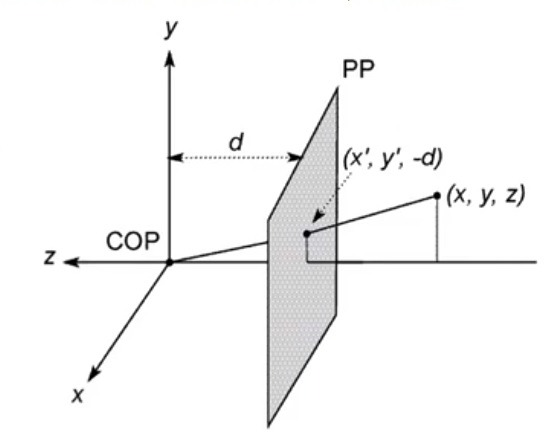
\includegraphics[scale=0.5]{Recursos/pinholeModel.jpg}
    \caption{Modelo de cámara pinhole}
    \label{pinholeModel}
\end{figure}
La razón del porque en el modelo presentado en la Figura \ref{pinholeModel} el plano de proyección se encuentra por delante del lente (a pesar de que en la realidad la luz ingresa a través del punto focal y luego impacta con el plano de imagen) es porque matemáticamente es más conveniente, debido a que de esta forma las imágenes no son invertidas.

Utilizando el teorema de Tales es posible determinar las proyecciones de los puntos en el plano de forma tal que se cumple la siguiente ecuación:
\begin{equation}
    (X, Y, Z) \longrightarrow (-d\frac{X}{Z}, -d\frac{Y}{Z}, -d)  \label{convert3Dto2Dpinhole}
\end{equation}
La operación realizada en la ecuación \ref{convert3Dto2Dpinhole}, permite proyectar los puntos del espacio 3D en el plano de imagen, dicha operación puede ser realizada mediante coordenadas homogéneas de la siguiente forma:
\begin{align}
            \begin{bmatrix}
            1 & 0 & 0 & 0\\
            0 & 1 & 0 & 0\\
            0 & 0 & 1/f & 0
            \end{bmatrix}
            \begin{bmatrix}
            x\\
            y\\
            z\\
            1
            \end{bmatrix}
            =
            \begin{bmatrix}
            x\\
            y\\
            z/f\\
            \end{bmatrix} \Rightarrow \left(-f\frac{X}{Z}, -f\frac{Y}{Z}\right)\label{convert3Dto2Dperspective}
\end{align}
A la forma en la que se proyecta en la ecuación \ref{convert3Dto2Dperspective} se le conoce como proyección de perspectiva y esta llega al mismo resultado que el de la ecuación \ref{convert3Dto2Dpinhole}, ya que $f$ es la distancia focal.
\\
El modelo de dos cámaras o modelo estéreo, es una extrapolación del modelo de pinhole. En general se pueden tener 3 casos en función de cómo se encuentren orientados los ejes de ambas cámaras: disposición convergente, disposición alineada y la disposición divergente, la tercera no permite llevar a cabo un análisis estéreo. En la figura \ref{estereoSystemParallel}, se puede observar el modelo geométrico de dos cámaras  cuando sus ejes ópticos son paralelos, a continuación se listan cada uno de los elementos relevantes:
\begin{itemize}
\item \textbf{Linea base:} es la distancia que separa los dos centros ópticos de ambas cámaras. Se denota B.
\item \textbf{distancia focal:} la distancia entre el plano de imagen y los centros ópticos. Se denota $f$.
\item\textbf{ El punto P:} corresponde con la distancia Z en las coordenadas de los sistemas de cámaras, siempre es medida hasta el centro de proyección (COP) de cada cámara. 
\item \textbf{Plano epipolar de un punto P en el espacio:} En la Figura \ref{estereoSystemParallel3D} se observa el mismo sistema pero con tres dimensiones, en este el plano que contiene el punto P y cada uno de sus centros ópticos $COP_{L}$ y $COP_{R}$ es conocido como el plano epipolar.
\item\textbf{ Linea epipolar:} hay una por cada punto ($p_{l}$ y $p_{r}$), en el caso de la Figura \ref{estereoSystemParallel3D} solo existe una linea debido a que esta es la intersección del plano epipolar con cada una de las imágenes.
\end{itemize}
\begin{figure}[H]
     \centering
     \begin{subfigure}[b]{0.4\textwidth}
        \centering
        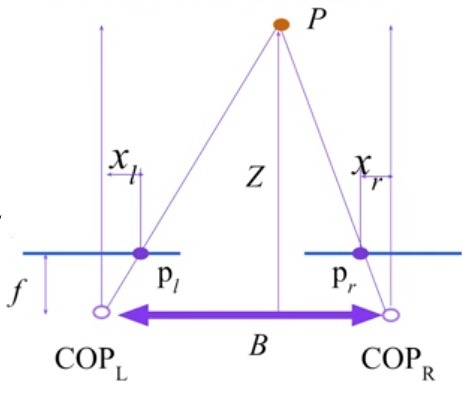
\includegraphics[scale=0.5]{Recursos/stereoGeometry.jpg}
        \caption{Representación del modelo de ejes alineados en el plano}
        \label{estereoSystemParallel}
     \end{subfigure}
     \hfill
     \begin{subfigure}[b]{0.4\textwidth}
         \centering
        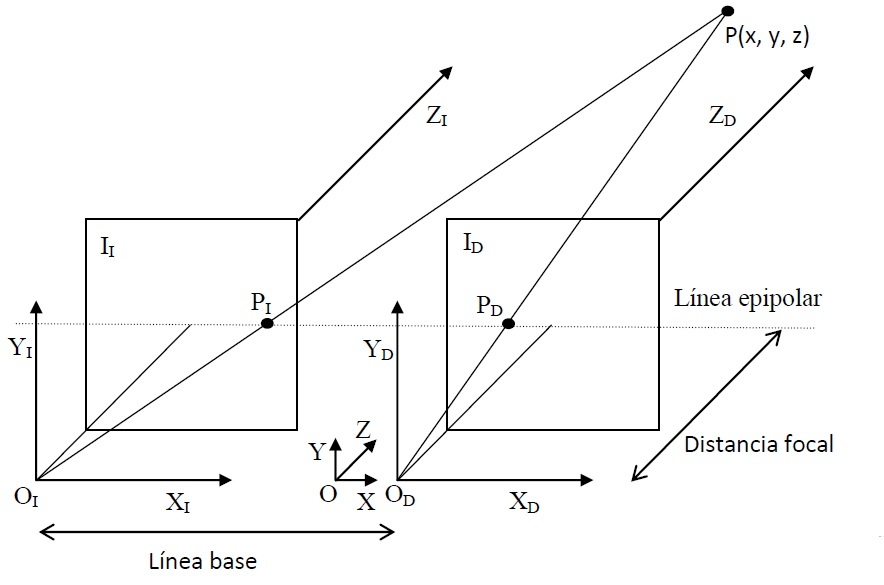
\includegraphics[scale=0.3]{Recursos/stereoGeometry3D.jpg}
        \caption{Representación del modelo de ejes alineados en el espacio}
        \label{estereoSystemParallel3D}
     \end{subfigure}
     \hfill
\caption{Modelo estéreo}
\label{stereoMODEL}
\end{figure}
Para el modelo de ejes alineados presentado en las Figuras \ref{estereoSystemParallel} y \ref{estereoSystemParallel3D}, es posible calcular las coordenadas de las proyecciones del punto P sobre cada una de las cámaras, utilizando el teorema de triángulos similares, de tal forma que su posición en el espacio estará dada por: 
\begin{align}
x_{p} = \frac{x_{l}\cdot B}{x_{l} - x_{r}}\\
y_{p} = \frac{y_{l}\cdot B}{x_{l} - x_{r}}\\
z_{p} = \frac{f\cdot B}{x_{l} - x_{r}}
\end{align}
La diferencia $x_{l} - x_{r}$ es conocida como disparidad.
\subsubsection{Extracción de las características}
En este paso se extraen los elementos que identifican a una imagen. De estos elementos, a su vez se tienen que extraer algunos atributos, los cuales se utilizarán en el siguiente paso. Por lo tanto, este paso está muy ligado al de correspondencia y al ser el paso de correspondencia el más importante de todos, primero se suele decidir qué método utilizar al realizar la correspondencia entre imágenes y según las características que se empleen, éstas serán las que se extraigan de las imágenes. Existen dos clases de técnicas para determinar la correspondencia entre dos imágenes estereoscópicas: las técnicas basadas en el área (“area-based”) y las técnicas basadas en las características (“feature-based”).
\\
Las técnicas basadas en área emplean la correlación cruzada entre patrones de intensidad en la vecindad local o vecindario de un píxel en una imagen, con patrones también de intensidad en una vecindad correspondiente a un píxel en la otra imagen del par estereoscópico. Por tanto, las técnicas basadas en el área utilizan la intensidad de los píxeles como característica esencial. Por otro lado las basadas en características se toman representaciones simbólicas obtenidas de las imágenes de intensidad en vez de utilizar las intensidades directamente. Algunas de las características cuyo uso está más extendido son: puntos de borde aislados, cadenas de puntos de bordes o regiones delimitadas por bordes.
\subsubsection{Correspondencia de las imágenes (características)}
Este paso puede tener como entradas pixeles o caracteristicas, de modo que con estas se calculen las profundidades a partir de la disparidad existente, la disparidad se puede entender como la diferencia entre las posiciones de las proyecciones en las imagenes y es representada por la siguiente expresión:
\begin{equation}
d = x_{l} - x_{r} = \frac{f\cdot B}{z_{p}}
\end{equation}
El problema de la disparidad es que existe cierta ambiguedad entre las imagenes. Habra puntos de caracteristicas similares en ambas imagenes y solo uno de esos puntos en cada uno de ellas son correspondientes entre si. De aqui la importancia del paso previo y es que en aquel paso se determina el conjunto inicial de caracteristicas faciles de distingir del resto de pixeles en las imagenes (esquinas, bordes, etc) y que serviran para inicializar el proceso de correspondencia. En la correspondencia se filtraran por medio de un conjunto de restricciones que vayan delimitando y reduciendo la ambiguedad de los posibles pares de proyecciones que se iran conjugando.
\\
Las restricciones pueden ser de tres tipos:
\begin{itemize}
\item\textbf{ Restricciones geométricas}: son aquellas impuestas por el sistema de visión estéreo. Entre todas ellas se destacan la restricción epipolar, la cual consiste en que las imágenes de una misma entidad 3D deben proyectarse sobre la misma línea epipolar. Esta restricción se deriva de la geometría de las cámaras y requiere que las mismas estén alineadas. Y la restricción de unicidad implica, que para cada característica en una imagen debe haber una única característica en la otra imagen, salvo que se produzca una oclusión y no haya correspondencia de alguna característica.
\item \textbf{Físicas y basadas en propiedades de la escena:} Dependen de la naturaleza de los objetos. Hacen  referencia a iluminaciones, superficies, formas, etc. Algunas de las mas usadas son la de ordenación, donde dadas dos características en una determinada imagen, por ejemplo la izquierda, situada una a la derecha de la otra, esta restricción supone que este mismo orden se mantiene en la imagen derecha para sus respectivas características homólogas. Y la restricción de continuidad límite de disparidad, asume que las variaciones de disparidad en la imagen son generalmente suaves, es decir que si consideramos un mapa de disparidad éste se presenta continuo salvo en unas pocas discontinuidades.
\end{itemize}
\subsubsection{Determinación de la distancia (profundidad)}
Una vez que se ha hecho corresponder los elementos que aparecen en la imagen izquierda con los elementos en la imagen derecha, la determinación de la profundidad es un proceso relativamente sencillo, reduciéndose a una simple triangulación. Sin embargo en algunas ocasiones, cuando se intenta hallar la distancia a la que se encuentra una característica, se presentan algunas dificultades debidas a una falta de precisión o una escasa fiabilidad cuando se intentó encontrar la correspondencia.
\\
Debido a las restricciones de epipolares, las proyecciones de un objeto real en cada una de las imágenes solamente se diferenciarán en la coordenada x de sus sistemas de referencia relativos, ya que la coordenada y será idéntica. De forma que dos elementos de las imágenes, que representan al mismo objeto, solo tendrán desplazamiento horizontal. Exactamente este desplazamiento es lo que hemos llamado disparidad.
\subsubsection{Interpolación}
Es un paso que no siempre es aplicado y se utiliza cuando se emplea el enfoque basado en características, ya que es cuando la información sobre distancias puede ser
insuficiente. Normalmente las aplicaciones requieren de mapas de profundidad más o
menos densos. Que un mapa de profundidad sea denso significa que hay mucha
información sobre la distancia a la que se encuentran los elementos de la escena por unidad de superficie, frente a un mapa de superficie disperso en el que la información que se dispone por unidad de superficie es menor. La densidad de un mapa es un valor que se puede cuantificar más o menos, pero que se considere lo suficientemente denso o no depende únicamente de la aplicación. Por ejemplo en el caso de un mapa de disparidad, donde cada píxel de la imagen capturada se disponga de un valor de la distancia a la que se encuentra ese punto de la cámara en la escena
tridimensional, se puede considerar muy denso.
\\
Sin embargo, en el caso de los métodos de correspondencia basados en características se suele llegar a mapas de disparidad dispersos, porque las características que tienen las imágenes suelen estar diseminadas y distribuidas irregularmente. Los métodos de correspondencia basados en el área son más apropiados que los métodos de correlación basados en las características si se quiere obtener un mapa de profundidades denso, aunque la información de los métodos basados en las características sea más fiable. La información de los métodos basados en el área suele ser menos fiable por problemas tales como la existencia de zonas donde el brillo es muy uniforme y no se puede realizar una correspondencia con certeza.
\\
Para solucionar estos problemas se emplea la interpolación, interpretando al mapa de disparidad, como un muestreo de una función de profundidad continua y utilizando el método de interpolación tradicional para hallar una función continua que la aproxime. Así se obtendría una función con la que obtener la profundidad para cualquier punto de espacio tridimensional, consiguiendo transformar un mapa de profundidad disperso en denso. Algunos de los métodos empleados para interpolar son: la interpolación de Lagrange, la interpolación de Hermite, interpolación mediante Splines, o mediante wavelets.
\subsection{Enfoque basado en Aprendizaje}
Los métodos basados en el aprendizaje pueden separarse en dos clases:
\begin{itemize}
    \item Las que imitan las técnicas de correspondencia estéreo, aprendiendo explícitamente cómo hacer coincidir los píxeles de la imagen de entrada de una cámara con los de la otra, para luego convertirlos en un flujo óptico o un mapa de disparidad y finalmente transformar cualquiera de los anteriores en su valor respectivo de profundidad. Esta estrategia posee tres módulos básicos: módulo de extracción, coincidencia de características y un modulo de agregación de costos, por ultimo se realiza la estimación de disparidad / profundidad (Ver Figura \ref{mimicStereo}). Es importante resaltar que esta estrategia se caracteriza porque cada modulo es entrenado independientemente de los otros \cite{laga2020survey}.
    \begin{figure}[H]
        \centering
        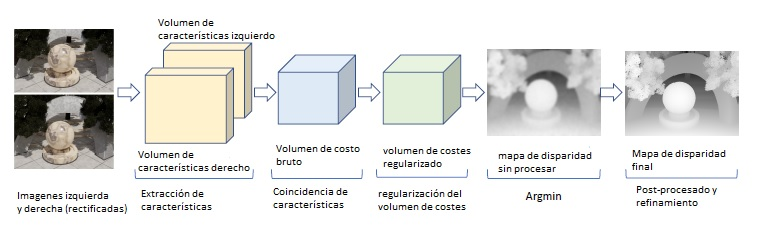
\includegraphics[scale=0.6]{Recursos/mimicStereo.jpg}
        \caption{Los componentes básicos para un proceso de correspondencia estéreo.}
        \label{mimicStereo}
    \end{figure}
    \item Las que resuelven el problema de correspondencia utilizando una ``pipeline'' o cadena de procesos que se puede entrenar de extremo a extremo. Esta categoría puede ser subdividida en dos tipos: aquellos métodos que formularon la estimación de profundidad como un problema de regresión. En otras palabras, el mapa de profundidad se infiere directamente de la entrada sin características que coincidan explícitamente a través de las vistas de ambas cámaras. Estos métodos son simples y rápidos en tiempo de ejecución, sin embargo; requieren una gran cantidad de datos de entrenamiento, el cual puede ser difícil de obtener. Por otro lado lo métodos que pertenecen a la segunda clase, imitan el canal de emparejamiento estéreo tradicional rompiendo el problema en etapas compuestas por bloques diferenciables y permitiendo así la formación de principio a fin.
\end{itemize}
\section{Fundamentos del aprendizaje profundo o deep learning}
El aprendizaje profundo, es una rama del aprendizaje automático ó machine learning, que se caracteriza por poseer un conjunto de datos de entradas, ejemplos de una salida esperada por el sistema y una forma de medir cuando un algoritmo esta realizando adecuadamente su trabajo, este ultimo elemento es necesario, ya que permite determinar la distancia entre la salida actual del algoritmo y la salida esperada, la medición de la salida es usada como una señal de realimentación para así ajustar la forma en que el algoritmo funciona. A este ajuste se le conoce como ``aprendizaje''.
\\
La idea base de este sub-campo del machine learning, nace del interés de replicar en sistemas computacionales el comportamiento de las neuronas presentes en los seres vivos, las cuales son responsables del aprendizaje y sus inicios datan de  1958 cuando Rosenblatt desarrollo el perceptron (Ver Figura \ref{perceptron}).
\begin{figure}[H]
    \centering
    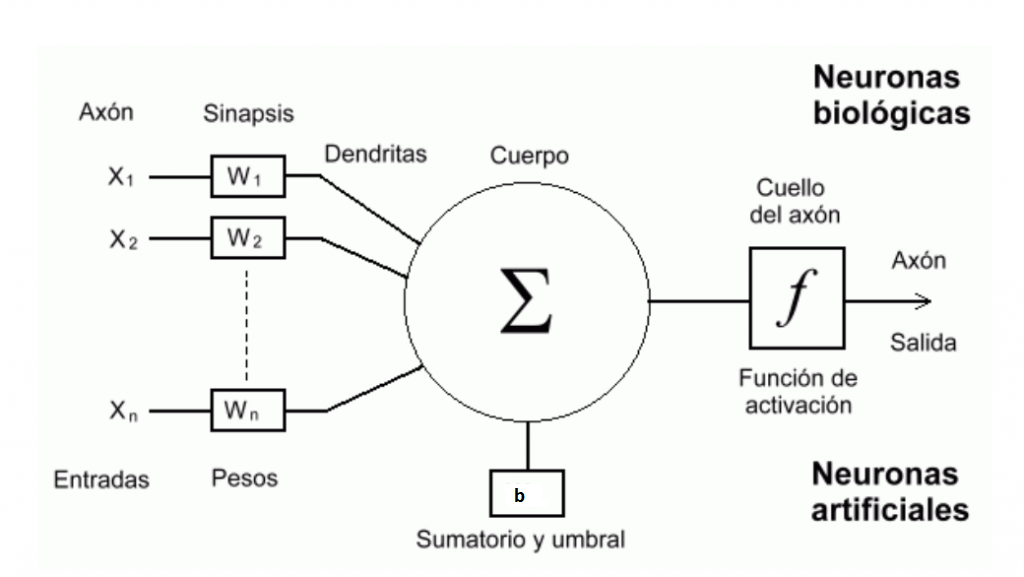
\includegraphics[scale=0.35]{Recursos/perceptron.png}
    \caption{Comparación de una neurona biológica con una neurona artificial}
    \label{perceptron}
\end{figure}
En comparación con otras técnicas de aprendizaje automático, que normalmente se basan en varias
etapas de pre-procesamiento para extraer características en las que se pueden construir clasificadores, el enfoque de aprendizaje profundo
generalmente se entrena de un extremo a otro, yendo directamente desde píxeles sin procesar hasta los resultados finales deseados \cite{Szeliski2020}.
\subsection{Elementos de las redes neuronales}
\subsubsection{Pesos y capas}
Una red neuronal profunda extiende la idea del perceptron (Ver Figura \ref{perceptron}) que utiliza una única neurona, a un grafo compuesto por miles de neuronas interconectadas. En la Figura \ref{NeuralNetworkArq} cada circulo corresponde con una neurona cuya salida estará dada por la siguiente expresión:
\begin{equation}
    s_{i} = w_{i}^{T} x_{i} + b_{i} \label{ponderedSum}
\end{equation}
el resultado de las sumas ponderadas (ecuación \ref{ponderedSum}) de cada neurona pasa por una función de activación no linear que redistribuirá los valores en un rango acotado:
\begin{equation}
    y_{i} = h(s_{i})
\end{equation}
En la ecuación \ref{ponderedSum}, los valores de $x_{i}$ son las entradas de de la i-esima neurona, $w_{i}$ y $b_{i}$ son parámetros que se van ajustando en el proceso de aprendizaje y corresponden con los pesos y el bias respectivamente. 
\begin{figure}[H]
    \centering
    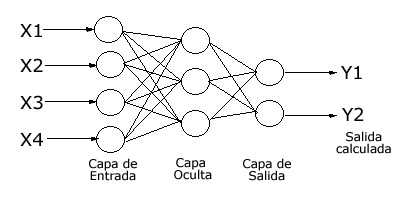
\includegraphics{Recursos/NeuralNetwork.jpg}
    \caption{Arquitectura de una red neuronal multicapas}
    \label{NeuralNetworkArq}
\end{figure}
A las capas de la Figura \ref{NeuralNetworkArq} se les conoce como ``fully conected'' (FC), debido a que todas las entradas de una capa están conectadas a todas sus salidas. Dado que las redes neuronales suelen estar organizadas en capas consecutivas, es posible agrupar cada neurona dentro de una capa en un vector, cuya combinación lineal se escribe como:
\begin{equation}
    s_{l} = w_{l}^{T} x_{l}
\end{equation}
donde $x_{l}$ son las entradas a la capa $l$, $W_{l}$ es una matriz de peso y $s_{l}$ es la suma ponderada, a la que se aplica una función de activación:
\begin{equation}
    x_{l+1} = y_{l} = h(s_{l)}
\end{equation}
Una red que consiste únicamente en capas FC, se le conoce como perceptron multicapa. 
\subsubsection{Funciones de activación}
Las funciones de activación se usan para propagar la salida de los nodos de una capa hacia la siguiente capa. Además este tipo de funciones permiten incorporar al modelo no linealidades, que permitirán que este se ajuste a cualquier distribución de datos. Algunas de las funciones de activación más comunes son:
\begin{itemize}
    \item \textbf{función logística o sigmoidea:} Este tipo de funciones permiten mitigar el efecto de ``outliers'' (valores atípicos que son numéricamente distantes del resto de los datos) en el entrenamiento del modelo. La imagen de este tipo de funciones suele estar contenida en los intervalos [0, 1]. Por lo que valores muy extremos siempre estarán cerca de los límites del intervalo de esa imagen. Su ecuación esta dada por:
    \begin{equation}
        h(x) = \frac{1}{1 + e^{-x}}
    \end{equation}
    \item \textbf{Tangente hiperbólica:} Es una función no lineal cuyo rango normalizado se encuentra entre [-1, 1] y su ventaja  es que puede manejar más fácilmente los números negativos. Su ecuación esta dada por:
    \begin{equation}
        h(x) = \frac{e^{x} - e^{-x}}{e^{x} + e^{-x}}
    \end{equation}
    \item \textbf{ReLu o rampa:} Es una de las funciones mas utilizadas en CNN y en redes profundas debido a que con ella se logran mejores resultados que con la sigmoidea y la hiperbólica, ya que en el procesamiento de imágenes los valores negativos  no son importantes y por lo tanto se establecen en 0. Pero los valores positivos después de la convolución deben pasar a la siguiente capa. En cambio si se emplean la hiperbólica o la sigmoidea,  la información se pierde ya que ambas funciones modificarán las entradas a un rango muy cerrado. Su ecuación esta dada por:
    \begin{equation}
        h(x) = max(0,x)
    \end{equation}
\end{itemize}
\subsubsection{Funciones de error}
Como se ha podido observar el proceso de aprendizaje de una red neuronal es de carácter iterativo, ya que, lo que se busca es ajustar un modelo a un conjunto de datos. Las funciones de error permiten medir la distancia a la que se encuentra un modelo del objetivo, de esta forma es posible tomar medidas adecuadas en la siguiente iteración, para así reducir el error hasta alcanzar valores mínimos. Dependiendo de la tarea a realizar se utilizan diferentes funciones de error. 
\\
Por ejemplo, en el caso de redes que utilicen como datos de entrada mapas de profundidad (mapas de disparidad) ó imágenes sin ruido, se suele realizar una regresión matemática que ajuste al modelo, por lo que es común utilizar la norma L2 como función de error
\begin{equation}
    E(w) = \sum_{n} E_{n}(w) = - \sum_{n} ||y_{n} - t_{n}||^{2}
\end{equation}
donde $y_{n}$ es la salida de la red para la muestra n y $t_{n}$ es el valor objetivo. Sin embargo, si son pocos los ``outliers'' en los datos de entrenamiento, o si los errores graves no son tan dañinos como para merecer una penalización cuadrática, se pueden utilizar normas más robustas como la L1
\begin{equation}
    E(w) = \sum_{n} E_{n}(w) = - \sum_{n} ||y_{n} - t_{n}||
\end{equation}
Cabe resaltar que no son las únicas funciones de error utilizadas en el campo de visión estéreo, pues existen variaciones, como en el trabajo realizado por Sizhang Dai y Weibing Huang en marzo del 2020 \cite{dai2020atvsnet} donde usan el error absoluto medio.
\subsubsection{Técnicas para la optimización de la red}
Cuando se entrena una red se emplean diversas técnicas que mejoran los resultados de la misma, o permiten que las redes neuronales no sufran de ``overfitting'' (sobre ajuste) para así poder generalizar mejor. A continuación se detallaran algunas de las técnicas mas empleadas así como lo es el ``dropout'' y la normalización del lote.
\begin{itemize}
    \item \textbf{Regularización:} es una técnica que surge cuando se optimizan los pesos dentro de una red neuronal, los pesos se vuelven más pequeños, a este fenómeno se le conoce como decaimiento de los pesos y es un problema debido a que al pasar por la función de activación un valor de suma ponderada muy cercano a 0, es mucho mas difícil para el algoritmo del descenso al gradiente desplazar el valor de ese peso a su óptimo. En la practica, valores muy pequeños se traducen a coeficientes con muchos decimales y esto es sinónimo de ``overfitting'', para solucionar esto se aplica regularización a la función de error, lo que penaliza en mayor medida a los pesos con largos coeficientes. A continuación se presentan las regularizaciones L1 y L2 respectivamente.
    \begin{align}
          E(w)_{L1} = - \sum_{n} ||y_{n} - t_{n}|| + \lambda \sum_{i} |w_{i}|\\
          E(w)_{L2} = - \sum_{n} ||y_{n} - t_{n}|| + \lambda \sum_{i} w_{i}^{2}\\
    \end{align}
    El valor de $\lambda$ corresponde con cuanto se quieren penalizar los coeficientes de los pesos $w_{i}$.
    \item \textbf{Dropout:} es una técnica aplicada a todas las neuronas de una capa, consiste en que a cada neurona de la capa en cuestión tendrá asociada una probabilidad de desactivación que puede estar entre 0 y 100\%, por lo que la red tendría un funcionamiento como el de la Figura \ref{dropout}.
    \begin{figure}[H]
        \centering
        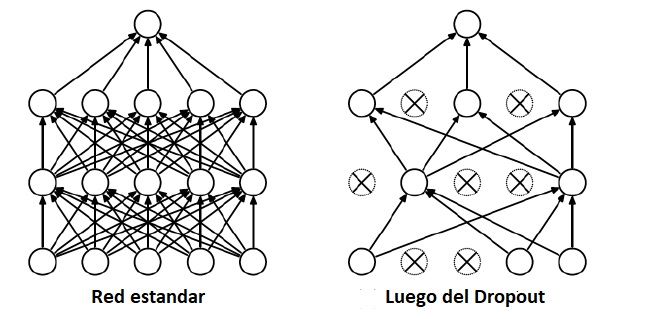
\includegraphics[scale=0.7]{Recursos/Dropout.jpg}
        \caption{Efecto del Dropout en el entrenamiento}
        \label{dropout}
    \end{figure}
    Colocar neuronas aleatoriamente a cero inyecta ruido en el proceso de formación y también evita que la red se especialice demasiado neuronas a muestras o tareas particulares, las cuales pueden ayudar a reducir el sobreajuste y mejorar la generalización.
    \item \textbf{Aumento del conjunto de datos:} Otra técnica poderosa para reducir el ajuste excesivo es agregar más muestras de entrenamiento perturbando las entradas y / o salidas de las muestras que ya han sido recolectadas. Esta técnica es eficaz en tareas de clasificación de imágenes, ya que es caro obtener ejemplos etiquetados, y también dado que las clases de imágenes no deben cambiar bajo pequeñas perturbaciones.
\end{itemize}
\subsubsection{Algoritmo de backpropagation}
Propuesto en 1986 por  Rumelhart, Hinton y Williams, es el responsable de que una red neuronal sea capaz de auto ajustar sus parámetros para así aprender una representación interna de la información que estaba procesando. Para su ejecución se requiere de un algoritmo conocido como descenso al gradiente, el cual consiste en que en cada iteración del entrenamiento se evalué el error del modelo y se calculen las derivadas parciales (gradientes) de dicho error, los gradientes indicaran la pendiente de la función hacia donde el error incrementa, por lo que para reducir el error en cada iteración, es necesario substraer el vector de gradientes al resultado final. 
\\
No obstante, debido a la estructura de una red neuronal, los valores de los parámetros en las capas posteriores dependen de las capas previas y a su vez de las conexiones entre neuronas, por lo que calcular el gradiente de forma directa no es una opción, la solución es utilizar el descenso del gradiente para optimizar la función de coste (función de error) empleando la técnica de de backpropagation para calcular el vector de gradientes dentro de la complejidad de la arquitectura de la red. 
\\
El funcionamiento de este algoritmo parte de analizar desde el final de la red con la señal de error hacia las primeras capas, la razón del porque se va desde la ultima capa hacia la primera capa, es que en una red neuronal el error de las capas anteriores depende directamente del error de las capas posteriores, teniendo en cuenta este hecho, es posible determinar cual es el efecto de cada neurona en el resultado final mediante la retro propagación de errores, de este modo es posible computar cuanto hay que modificar cada parámetro en cada neurona. Además una vez aplicados los errores a las neuronas de la capa de turno se puede proceder a repetir el mismo proceso previo como si este fuera el error de la red; es decir, asumiendo que la capa de turno es la nueva ultima capa, así aplicar backpropagation es operar siempre de forma recursiva capa tras capa moviendo el error hacia atrás. Entonces al alcanzar la primera capa se habrá obtenido cual es el error para cada neurona y para cada uno de sus parámetros, dichos errores son usados para calcular las derivadas parciales de cada parámetro de la red, conformado así el vector de gradientes al cual se le aplica el descenso al gradiente para lograr minimizar el error. 
\subsection{Redes neuronales convolucionales ó Convolutional Neural Networks (CNN)}
Es una arquitectura de red empleada en el procesamiento de imágenes, cuya principal ventaja respecto a las redes estudiadas previamente, es su eficiencia al momento del entrenamiento, ya que la cantidad de parámetros a ajustar se reduce considerablemente. A diferencia de una red de capas FC las capas de las redes CNN consisten en un conjunto de filtros que se van ajustando a medida que avanza el aprendizaje, cada filtro suele ser pequeño espacialmente (tanto en ancho como en alto)  respecto a las dimensiones de la imagen de entrada, pero estos se extienden a través de todas las dimensiones del volumen de entrada, se le conoce como volumen de entrada debido a que una imagen con los 3 canales (RGB) corresponde con un tensor de dimensiones  $WxHxD$ (ancho x alto x profundidad). Al introducir una imagen en la red se desliza (mas precisamente, se realiza la convolución) cada filtro a través de todo el ancho y alto del volumen de entrada y se calculan los productos escalares entre las entradas del filtro y la entrada en cualquier posición.  A medida que se desliza el filtro sobre el ancho y el alto del volumen de entrada, se producirá un mapa de activación bidimensional o mapa de características, que da las respuestas de ese filtro en cada posición espacial (Ver Figura \ref{fowardPassCNN}).
\begin{figure}[H]
    \centering
    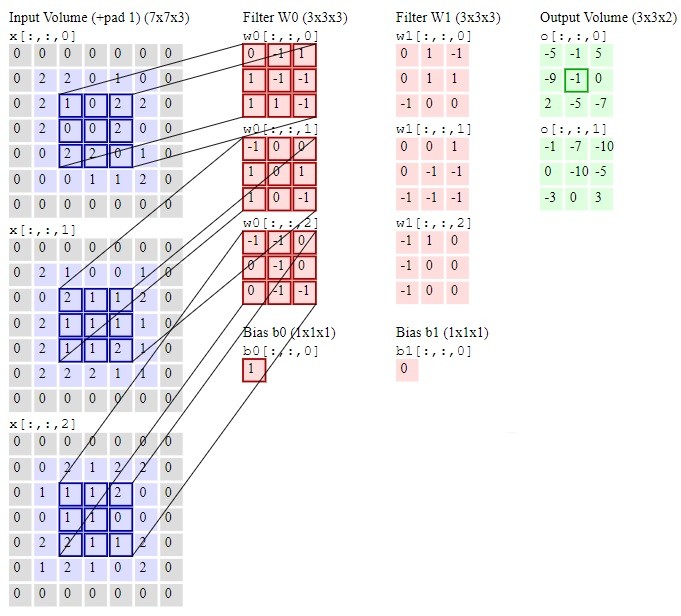
\includegraphics[scale=0.7]{Recursos/fowardPassCNN.jpg}
    \caption{Convolución entre el volumen de entrada de dimensiones 7x7x3 y dos filtros de dimensiones 3x3x3}
    \label{fowardPassCNN}
\end{figure}
De forma intuitiva, la red aprenderá filtros que se activan cuando ven algún tipo de característica visual, como un borde de alguna orientación o una mancha de algún color en la primera capa, o eventualmente patrones enteros en forma de panal o rueda en capas superiores de la red. De este modo se tendrá un conjunto completo de filtros en cada capa, en lugar de neuronas y cada uno de ellos producirá un mapa de activación bidimensional separado. Se Apilaran estos mapas de activación a lo largo de la dimensión de profundidad generando así el volumen de salida\cite{CS231n}.
\\ 
En las CNN se suelen emplear dos tipos de capas, aquellas donde se realiza la convolución, las cuales fueron descritas previamente y las capas de agrupación o ``polling layers'', estas son insertadas periódicamente entre capas de convolución con el fin de reducir progresivamente el tamaño espacial de la representación para así disminuir la cantidad de parámetros y cálculos en la red y, por lo tanto, controlar también el ``overfitting''. La capa de agrupación funciona de forma independiente  en cada segmento de profundidad de la entrada y la redimensiona espacialmente, utilizando la operación MAX. La forma más común es una capa de agrupación con filtros de tamaño 2x2 aplicados con un paso de 2, por lo que con estos parámetros la operación MAX tomaría el valor máximo entre 4 números en una región de 2x2 (Ver Figura \ref{maxPooling}). De manera más general, la capa de agrupación:
\begin{itemize}
    \item Acepta un volumen de dimensiones $W_{1}xH_{1}xD_{1}$
    \item Requiere dos hiperparámetros:
    \begin{itemize}
        \item Su extensión espacial ``F''
        \item El paso o zancada ``S''
    \end{itemize}
    \item Produce un volumen $W_{2}xH_{2}xD_{2}$ donde:
    \begin{itemize}
        \item $W_{2}$ $=$ $(W_{1}-F)/S+1$
        \item $H_{2}$ $=$ $(H_{1}-F)/S+1$
        \item $D_{2}$ $=$ $D_{1}$
    \end{itemize}
    \item Introduce cero parámetros ya que calcula una función fija de la entrada
    \item Para las capas de agrupación, no es común rellenar la entrada con relleno de ceros, como en el caso de una capa de convolución.
\end{itemize}
\begin{figure}[H]
    \centering
    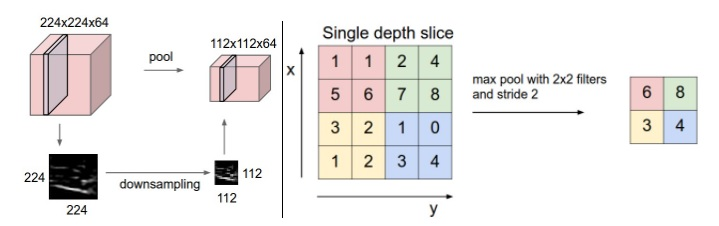
\includegraphics[scale=0.6]{Recursos/maxPolling.jpg}
    \caption{Capa de agrupación para un volumen de entrada de 224x224x64 con F = 2, P = 2 y un volumen de salida de 112x112x32}
    \label{maxPooling}
\end{figure}
\subsection{Hiperparámetros de las redes CNN}
Son las variables que rigen el proceso de entrenamiento en sí, es decir; son variables de configuración. En el caso de las capas de convolución se tienen:
\begin{enumerate}
    \item La profundidad del volumen de salida: corresponde a la cantidad de filtros a usar en cada capa y se identifica por $D_{n}$ donde $n$ es el numero de la capa en cuestión. Sin embargo, también puede identificarse mediante $K$.
    \item El campo receptivo de la neurona: es equivalente al tamaño del filtro y se identifica mediante $F$.
    \item El paso o zancada: corresponde con la cantidad de pixeles por las que se desliza el filtro al momento de realizar la convolución, se identifica mediante la letra $S$. Por ejemplo cuando el paso es 1, los filtros se desplazan un píxel a la vez. En el caso de ser 2 los filtros saltan 2 píxeles a la vez a medida que se deslizan por el volumen de entrada, de esta forma se producirán volúmenes de salida más pequeños espacialmente.
    \item El relleno: hay casos donde sera conveniente rellenar el volumen de entrada con ceros alrededor del borde, como es el caso de la Figura \ref{fowardPassCNN}. Por lo tanto el tamaño del relleno de ceros es un hiperparámetro que  permitirá controlar el tamaño espacial de los volúmenes de salida, aunque su aplicación más común es la de preservar exactamente el tamaño espacial del volumen de entrada para que el ancho de entrada y salida y la altura sean los mismos.
    \item Dilatación: este parámetro permite tener filtros que tengan espacios entre cada celda, por ejemplo; en el caso de una dimensión un filtro $w$ de tamaño 3 calcularía sobre la entrada $x$ lo siguiente:  $w [0] * x [0] + w [1] * x [1] + w [2] * x [2]$ . Este es en el caso de que no exista dilatación (dilatación = 0). Para la dilatación = 1, el filtro calcularía $w [0] * x [0] + w [1] * x [2] + w [2] * x [4]$; En otras palabras, hay una brecha de 1 entre las aplicaciones.  Esto puede ser muy útil en algunas configuraciones para usar junto con filtros de dilatación 0 porque le permite fusionar información espacial a través de las entradas de manera mucho más agresiva con menos capas.
\end{enumerate}
De acuerdo con los hiperparámetros, una capa convolucional se caracteriza por:
\begin{itemize}
    \item Acepta un volumen de dimensiones $W_{1}xH_{1}xD_{1}$.
    \item Requiere 4 hiperparámetros:
    \begin{itemize}
        \item El numero de filtros ``K''
        \item La extensión de los filtros ``F''
        \item El paso ``S''
        \item la cantidad de relleno ``P''.
    \end{itemize}
    \item Produce un volumen $W_{2}xH_{2}xD_{2}$ donde:
    \begin{itemize}
        \item $W_{2}$ $=$ $(W_{1} - F + 2P)/S+1$
        \item $H_{2}$ $=$ $(H_{1} - F + 2P)/S+1$
        \item $D_{2}$ $=$ $K$
    \end{itemize}
\end{itemize}
